\section{Legame chimico}
Il \textbf{legame chimico} è l'unione tra atomi, uguali o diversi, che da luogo a uno stato più stabile da punto di vista energetico.

Per creare un legame abbiamo bisogno che gli \textbf{elettroni di valenza} di un elemento, ovvero quelli del guscio più esterno che sono responsabili dei legami e delle reazioni chimiche, vengono trasferiti totalmente o condivisi con un altro elemento affinché entrambi raggiungono l'ottetto.

Per rappresentare gli elettroni di valenza di un atomo si utilizza la \textbf{struttura di Lewis}. Questa rappresentazione si basa sul scrivere intorno al simbolo dell'elemento tanti puntini quanti sono gli elettroni di valenza.

\begin{table}[H]
	\centering
	\setlength{\tabcolsep}{15pt} % for the horizontal padding
	\renewcommand{\arraystretch}{1.5}% for the vertical padding
	\begin{tabular}{cccccccc}
		\toprule
		1A                        & 2A                        & 3A                              & 4A                                     & 5A                                           & 6A                                           & 7A                                            & 8A                                            \\
		\midrule
		\charge{0:2pt=\.}{H}  &                           &                                 &                                        &                                              &                                              &                                               & \charge{0:2pt=\:}{He}                     \\
		\charge{0:2pt=\.}{Li} & \charge{0:2pt=\:}{Be} & \charge{0:2pt=\:,90:2pt=\.}{B}  & \charge{0:2pt=\:,90:2pt=\.,180:2pt=\.}{C}  & \charge{0:2pt=\:,90:2pt=\.,180:2pt=\.,270:2pt=\.}{N} & \charge{0:2pt=\:,90:2pt=\.,180:2pt=\:,270:2pt=\.}{O} & \charge{0:2pt=\:,90:2pt=\.,180:2pt=\.,270:2pt=\:}{F}  & \charge{0:2pt=\:,90:2pt=\:,180:2pt=\:,270:2pt=\:}{Ne} \\
		\charge{0:2pt=\.}{Na} & \charge{0:2pt=\:}{Mg} & \charge{0:2pt=\:,90:2pt=\.}{Al} & \charge{0:2pt=\:,90:2pt=\.,180:2pt=\.}{Si} & \charge{0:2pt=\:,90:2pt=\.,180:2pt=\.,270:2pt=\.}{P} & \charge{0:2pt=\:,90:2pt=\.,180:2pt=\:,270:2pt=\.}{S} & \charge{0:2pt=\:,90:2pt=\.,180:2pt=\.,270:2pt=\:}{Cl} & \charge{0:2pt=\:,90:2pt=\:,180:2pt=\:,270:2pt=\:}{Ar} \\
		\bottomrule
	\end{tabular}
	\caption{Strutture di Lewis dei primi diciotto elementi della Tavola Periodica}
\end{table}

\subsection{Legame ionico}
Un \textbf{legame ionico} si forma tra un metallo e non metallo, mediante il trasferimento di elettroni dall'atomo meno elettronegativo (\textbf{catione}) all'atomo più elettronegativo (\textbf{anione}). Generalmente, la differenza di elettronegatività fra i due atomi è maggiore di 1,9.
\begin{reactions*}
	\charge{0:2pt=\.}{Na} \+ \charge{0:2pt=\:,90:2pt=\:,180:2pt=\.,270:2pt=\:}{Cl} \arrow
	\charge{30:3pt=\chargeColor{+}}{Na} \+ \charge{0:2pt=\:,90:2pt=\:,180:2pt=\:,270:2pt=\:,35:3pt=\chargeColor{-}}{Cl}
\end{reactions*}

\subsection{Legame covalente}
Un legame covalente si forma quando vengono condivise coppie di elettroni tra i due atomi e la differenza di elettronegatività fra i due atomi è minore di 1,9. Di legami covalenti ne esistono tre tipi:
\begin{description}
	\item[\qquad Covalente Puro:] Quando il legame si forma tra due atomi della stessa specie chimica.
		\begin{reactions*}
			\charge{0:2pt=\.,90:2pt=\:,180:2pt=\:,270:2pt=\:}{Cl} \+ \charge{0:2pt=\:,90:2pt=\:,180:2pt=\.,270:2pt=\:}{Cl}
			\arrow
			\chemfig{\charge{90:2pt=\:,180:2pt=\:,270:2pt=\:}{Cl}-\charge{0:2pt=\:,90:2pt=\:,270:2pt=\:}{Cl}}
		\end{reactions*}
	\item[\qquad Covalente Omopolare:] Quando il legame si forma tra due atomi con una differenza di elettronegatività minore 0,4.
		\begin{reactions*}
			\charge{0:2pt=\.,90:2pt=\.,180:2pt=\.,270:2pt=\.}{C} \+ 4\; \charge{180:2pt=\.}{H} \arrow
			\chemfig{H-C(-[2]H)(-[6]H)-H}
		\end{reactions*}
	\item[\qquad Covalente Polare:] Quando il legame si forma tra due atomi con una differenza di elettronegatività tra 0,4 e 1,9.
		\begin{reactions*}
			\charge{0:2pt=\.}{H} \+ \charge{0:2pt=\:,90:2pt=\:,180:2pt=\.,270:2pt=\:}{Cl} \arrow \chemfig{H-\charge{0:2pt=\:,90:2pt=\:,270:2pt=\:}{Cl}}
		\end{reactions*}
\end{description}

In un legame covalente polare si genera una parziale carica negativa sull'atomo più elettronegativo indicata con \(\delta-\) mentre si genera una parziale carica positiva indicata con \(\delta+\). Questa separazione di cariche genera un \textbf{momento di dipolo}.

Se le parziali cariche si trovano in posizione opposta nella molecola, il momento di dipolo si annulla e avremo una \textit{molecola apolare} mentre se le cariche si trovano in posizione diversa avremo una \textit{molecola polare}.


Questa polarità di legame covalente si può vedere tramite il \textit{modello di densità elettronica} dove il colore blu indica la presenza un carica \(\delta+\) mentre il colore rosso indica la presenza di un carica \(\delta-\).

\begin{figure}[H]
	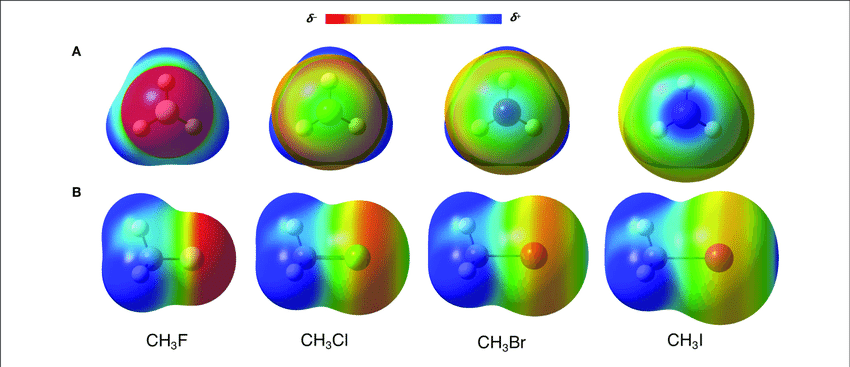
\includegraphics[width=\textwidth,trim={3cm 0 2cm 1cm},clip,]{immagini/electron density model.png}
	\caption{Alcune molecole raffigurate tramite modello di densità elettronica}
\end{figure}

Quando si combinano due atomi per formare una molecola, si sviluppa energia. Quella stessa energia servirà per rompere il legame. Questa energia prende il nome di \textbf{energia di legame} e varia da legame a legame. Un altro dato importante da ricordarsi è la \textbf{lunghezza di legame}, ovvero la distanza fra i due nuclei e ha come unità di misura {\AA}ngstr\"{o}m\footnote{\si{1 \angstrom} corrisponde a \si{0,1\pm} o \si{\qty{1e-12}\m}} (\si{\angstrom}).

\subsection{Disegnare strutture di Lewis di molecole e ioni}
Per rappresentare le molecole si utilizzano le strutture di Lewis. Le seguenti regole servono per disegnarle:
\begin{enumerate}
	\item Determina il numero di elettroni di valenza nelle molecole o ione
	\item Determina la sistemazione degli atomi nella molecola o ione
	\item  Sistema gli elettroni residui in coppie, in modo che ciascun atomo nella molecola o nello ione abbia un guscio di valenza completo
	\item Indica una coppia di \textbf{elettroni di legame} con una singola linea mentre una coppia di \textbf{ elettroni di non legame} con dei puntini
	\item Utilizza legami multipli dove necessario
\end{enumerate}
Nei composti organici neutri, si possono fare alcune generalizzazioni per alcuni elementi come:
\begin{itemize}
	\item \elementsymbol{1} ha un solo legame
	\item \elementsymbol{6} ha quattro legami
	\item \elementsymbol{7} ha tre legami e una coppia di non legame
	\item \elementsymbol{8} ha due legami e due coppie di non legame
	\item \elementsymbol{9}, \elementsymbol{Chlorine}, \elementsymbol{Bromine} e \elementsymbol{Iodine} hanno un solo legame e tre coppie di non legame
\end{itemize}

\subsection{Carica formale}
La \textbf{carica formale} è la carica di un atomo in uno ione poliatomico o in una molecola.
Per determinare la carica formale
\begin{enumerate}
	\item Scrivi una struttura di Lewis corretta per la molecola o ione
	\item Assegna a ciascun atomo tutti i suoi elettroni non condivisi (di non legame) e metà dei suoi elettroni condivisi (di legame)
	      \begin{equation*}
		      \text{Carica formale} \;=\;
		      \begin{matrix}
			      \text{Numero di elettroni}   \\
			      \text{di valenza nell'atomo} \\
			      \text{neutro non legato}
		      \end{matrix}
		      \;-\; \left(\;
		      \begin{matrix}
				      \text{Tutti gli elettroni} \\
				      \text{non condivisi}       \\
			      \end{matrix}
		      \;+\;
		      \begin{matrix}
				      \text{Metà degli} \\
				      \text{elettroni}  \\
				      \text{condivisi}
			      \end{matrix}\;
		      \right)
	      \end{equation*}
	\item Confronta questo numero con il numero di elettroni di valenza dell'atomo neutro non legato
	      \begin{itemize}
		      \item Se il numero è maggiore, l'atomo avrà una carica positiva
		      \item Se il numero è minore, l'atomo avrà carica negativa
	      \end{itemize}
\end{enumerate}

\begin{framed}
	\noindent\textbf{NOTA:}
	Una struttura di Lewis ha carica netta zero questo significa che nella struttura ci possono essere anche delle cariche che però si devono annullare a vicenda.
\end{framed}
